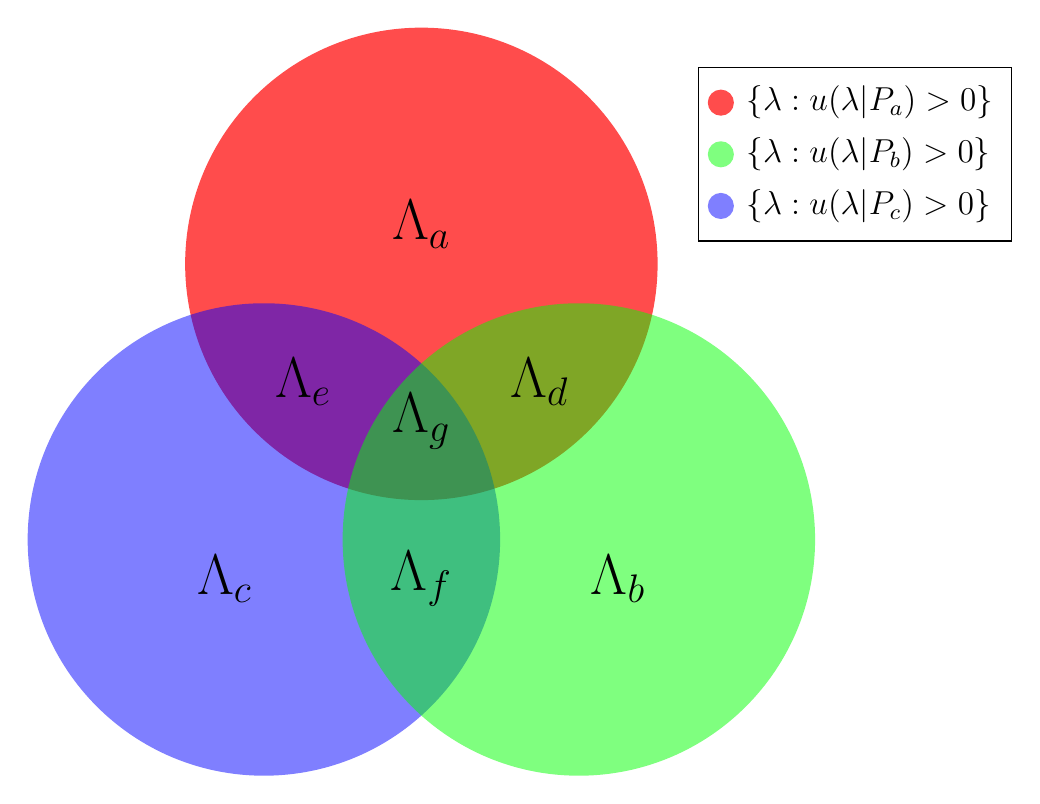
\begin{tikzpicture}[ blacknode/.style={},
  bluenode/.style={shape=circle, fill=blue, opacity=0.5, line width=2},
  greennode/.style={shape=circle,fill=green, opacity=0.5, line width=2},
  rednode/.style={shape=circle, fill=red, opacity=0.7, line width=2}
]

\node (v1) at (0,6.5) {};
\fill[red,fill opacity=0.7]  (v1) ellipse (3 and 3);
\node (v2) at (-2,3) {};
\fill[blue,fill opacity=0.5]  (v2) ellipse (3 and 3);
\node (v3) at (2,3) {};
\fill[green,fill opacity=0.5]  (v3) ellipse (3 and 3);


 


\matrix [draw,below left] at (7.5,9) {
  \node [rednode,label=right:{\large $\{\lambda:u(\lambda|P_a)>0\}$}] {}; \\
  \node [greennode,label=right:{\large $\{\lambda:u(\lambda|P_b)>0\}$}] {}; \\
  \node [bluenode,label=right:{\large $\{\lambda:u(\lambda|P_c)>0\}$}] {}; \\
};
\node at (0,7) {\huge $\Lambda_a$};
\node at (2.5,2.5) {\huge $\Lambda_b$};
\node at (-2.5,2.5) {\huge $\Lambda_c$};
\node at (1.5,5) {\huge $\Lambda_d$};
\node at (-1.5,5) {\huge $\Lambda_e$};
\node at (0,2.5) {\huge $\Lambda_f$};
\node at (0,4.5) {\huge $\Lambda_g$};

\end{tikzpicture}